\section*{Aufgabe 3}
\label{sec:3}

In dieser Aufgabe wurde das zweidimensionale DGSEM-Verfahren auf das Problem
\textit{Attacke im Häuserblock} mit den gegebenen Anfangsdaten angewendet.

Abbildungen \ref{abb:A31} und \ref{abb:A32} zeigen den Messverlauf des
Mikrophones in der Zeit für die beiden Simulationen mit jeweils $N=6$ und
$CFL=0.8$.

Die Anfangsdaten wurden wie folgt gesetzt:
\begin{align}
v_1 &= 0\\
v_2 &= \begin{cases}
1, \ (x,y)\in W\\
0, \ \text{sonst}
\end{cases}\\
p &= \begin{cases}
3\exp (\frac{1}{2}(\frac{(x-\frac{1}{2})^2+(y-\frac{1}{4})^2}{s}))+2, \ (x,y)\in W\\
2, \ \text{sonst}
\end{cases}
\end{align}
mit $W:=\{(x,y) | 0.4\leq x\leq 0.6 \; \wedge \; 0.1\leq y\leq 0.4\}$ und $s=10^{-2}$.

An den äußeren Rändern sind Dirichlet-Randbedingungen angenommen worden mit \\
$(v_1,v_2,p)^T = (0,0,2)^T$. Die Hauswände und der untere Rand werden als
reflektierende Ränder betrachtet. An einem reflektierenden Rand wird bei einem
Wert von $u=(v_1,v_2,p)^T$ der äußere Wert des entsprechenden Riemannproblems
auf den orthogonal zum Rand gespiegelten Wert gesetzt, z.B. an der y-Achse auf
$\^{u}=(v_1,-v_2,p)^T$.

\begin{figure}[H]
	\begin{center}
		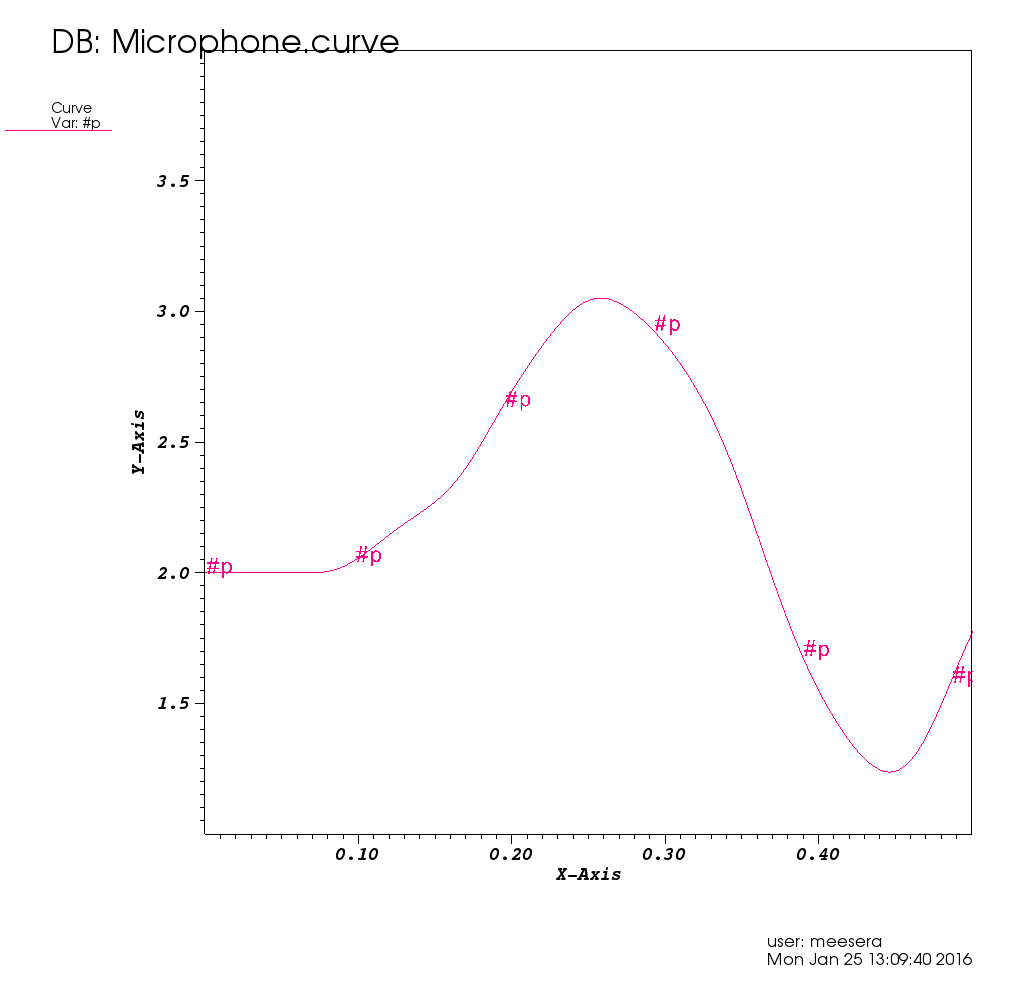
\includegraphics[width=0.8\textwidth]{img/Microphone_lowRes.png}
		\caption{Messverlauf des Mikrophones in der Zeit für eine Diskretisierung mit $100$ Zellen.}
		\label{abb:A31}
	\end{center}
\end{figure}

\begin{figure}[H]
	\begin{center}
		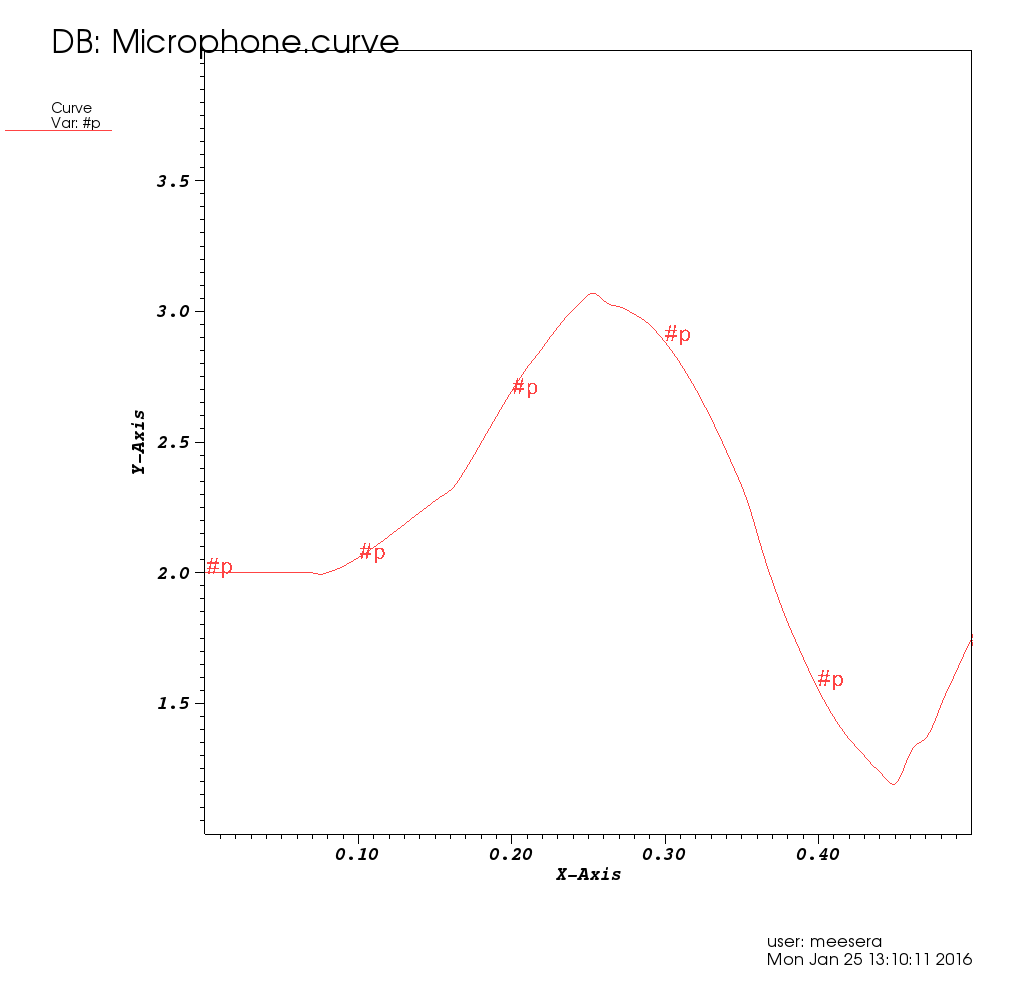
\includegraphics[width=0.8\textwidth]{img/Microphone_highRes.png}
		\caption{Messverlauf des Mikrophones in der Zeit für eine Diskretisierung mit $2500$ Zellen.}
		\label{abb:A32}
	\end{center}
\end{figure}

Es ist zu erkennen wie sich der Druck von dem gezündeten Böller ausbreitet und
dann das Mirkrophon erreicht. Danach wird er von den reflektierenden Wänden
wieder zurückgeworfen. Der Druck nimmt ab, bis er schließlich wieder zum
Ausgangsniveau zurückkehrt.

Der Druck auf dem gesamten Gebiet zum Zeitpunkt $t=0.5$ stellt sich wie in den
Abbildungen \ref{abb:A33} und \ref{abb:A34} dar.

\begin{figure}[H]
	\begin{center}
		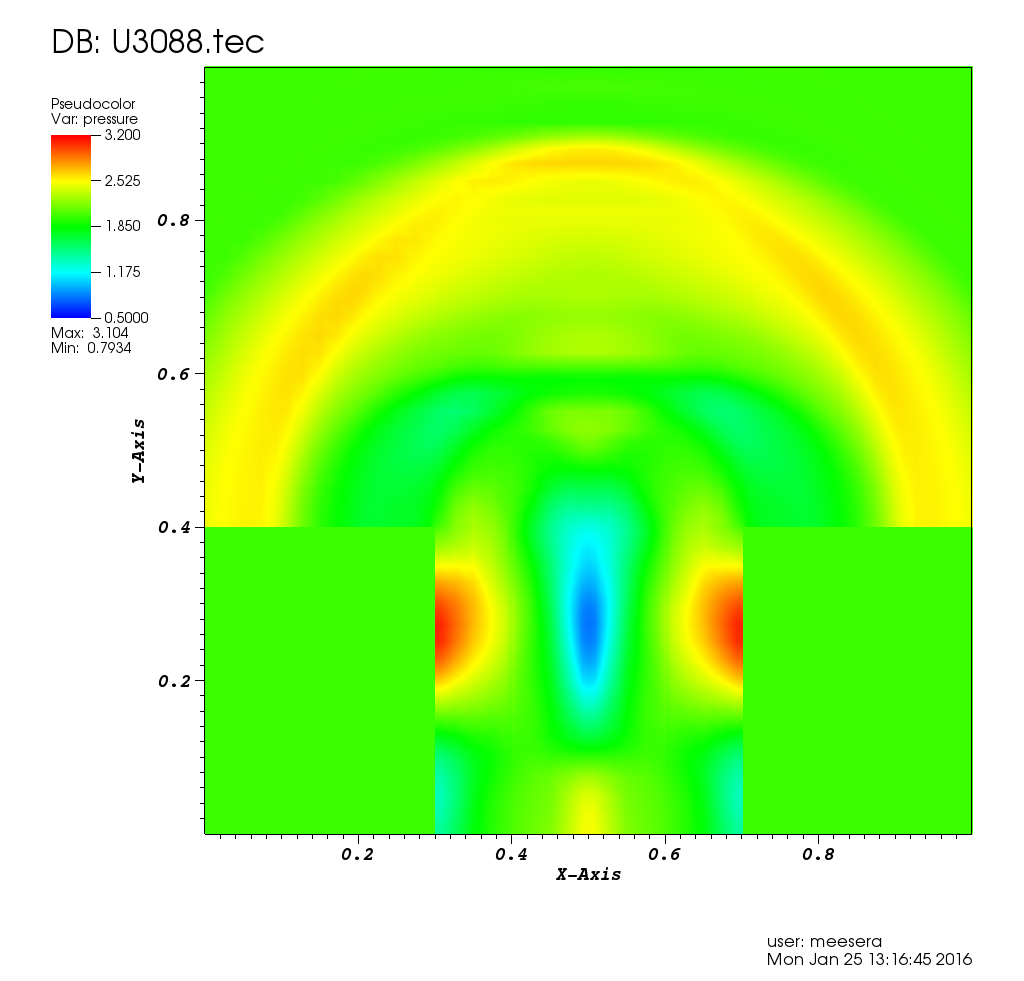
\includegraphics[width=0.8\textwidth]{img/Pressure_lowRes_scaled.png}
		\caption{Druck zum Zeitpunkt $t=0.5$ für eine Diskretisierung mit $100$ Zellen.}
		\label{abb:A33}
	\end{center}
\end{figure}

\begin{figure}[H]
	\begin{center}
		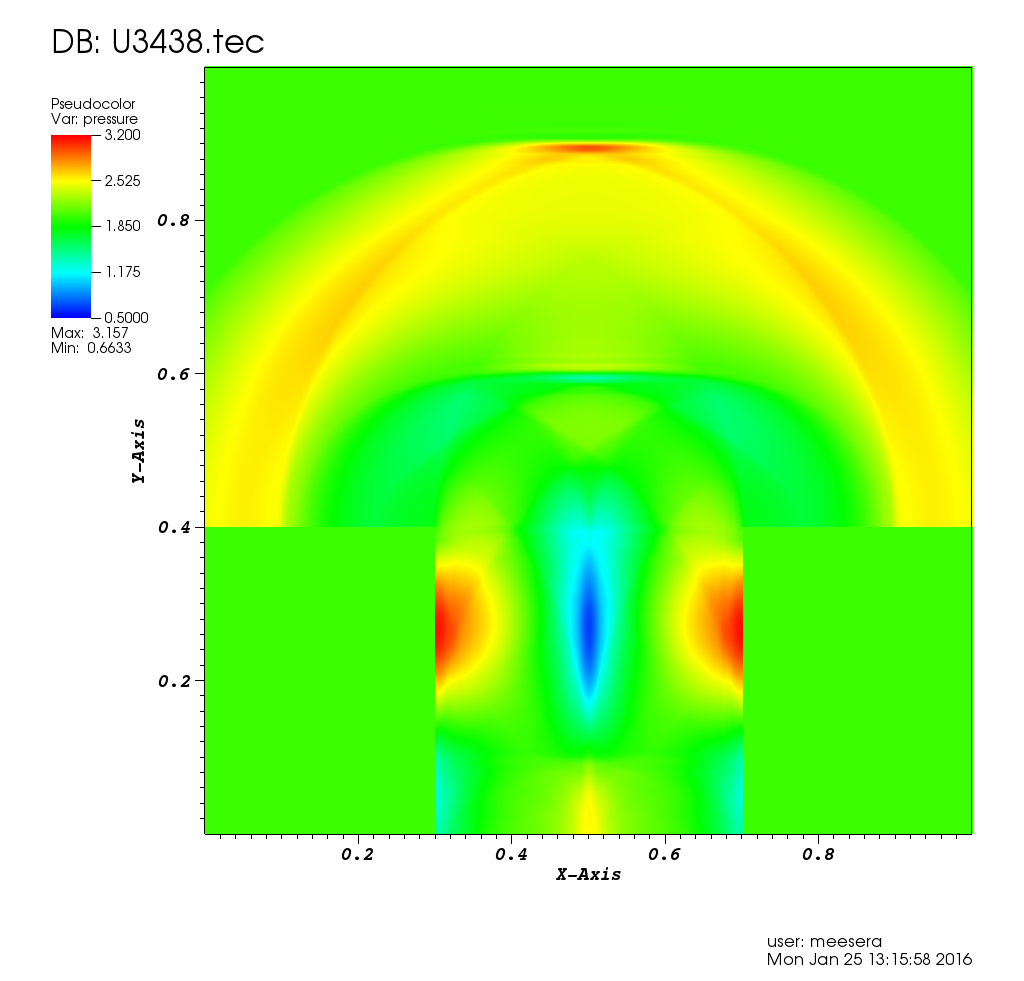
\includegraphics[width=0.8\textwidth]{img/Pressure_highRes_scaled.png}
		\caption{Druck zum Zeitpunkt $t=0.5$ für eine Diskretisierung mit $2500$ Zellen.}
		\label{abb:A34}
	\end{center}
\end{figure}

Man erkennt, das beide Diskretisierungen, fast gleiche Ergebnisse liefern.
Lediglich die Stoßwelle für 2500 Zellen erscheint stärker ausgeprägt und
scharfkantiger zu sein. Die spricht für eine höhere, und damit bessere
Auflösung des physikalischen Vorgangs. Auffällig ist jedoch die tiefrote
Stelle an der vordersten Spitze der Stoßwelle. Dies erscheint uns eher
unatürlich. Dies könnte ein numerisches Artefakt sein. Interessant ist auch das
Auftreten negativer Druckwerte, welche durch Überschwingen des System enstehen.
Ein höherer Normaldruck, in diesem Projekt beträgt er $p_{normal} = 2$, könnte
das verhindern.
